% =================================================================================================
% File:			client_tier/model.tex
% Description:	Defiinisce la sezione relativa al front-end dell'applicazione
% Created:		2015-04-07
% Author:		Tesser Paolo
% Email:		tesser.paolo@mashup-unipd.it
% =================================================================================================
% Modification History:
% Version		Modifier Date		Change											Author
% 0.0.1 		2015-04-07 			creato scheletro								Tesser Paolo
% =================================================================================================
%
%

% CONTENUTO DEL CAPITOLO


\subsubsection{client::model} % (fold)
\label{ssub:bdsm_app_client_model}
\begin{figure}[htbp]
	\centering
	\centerline{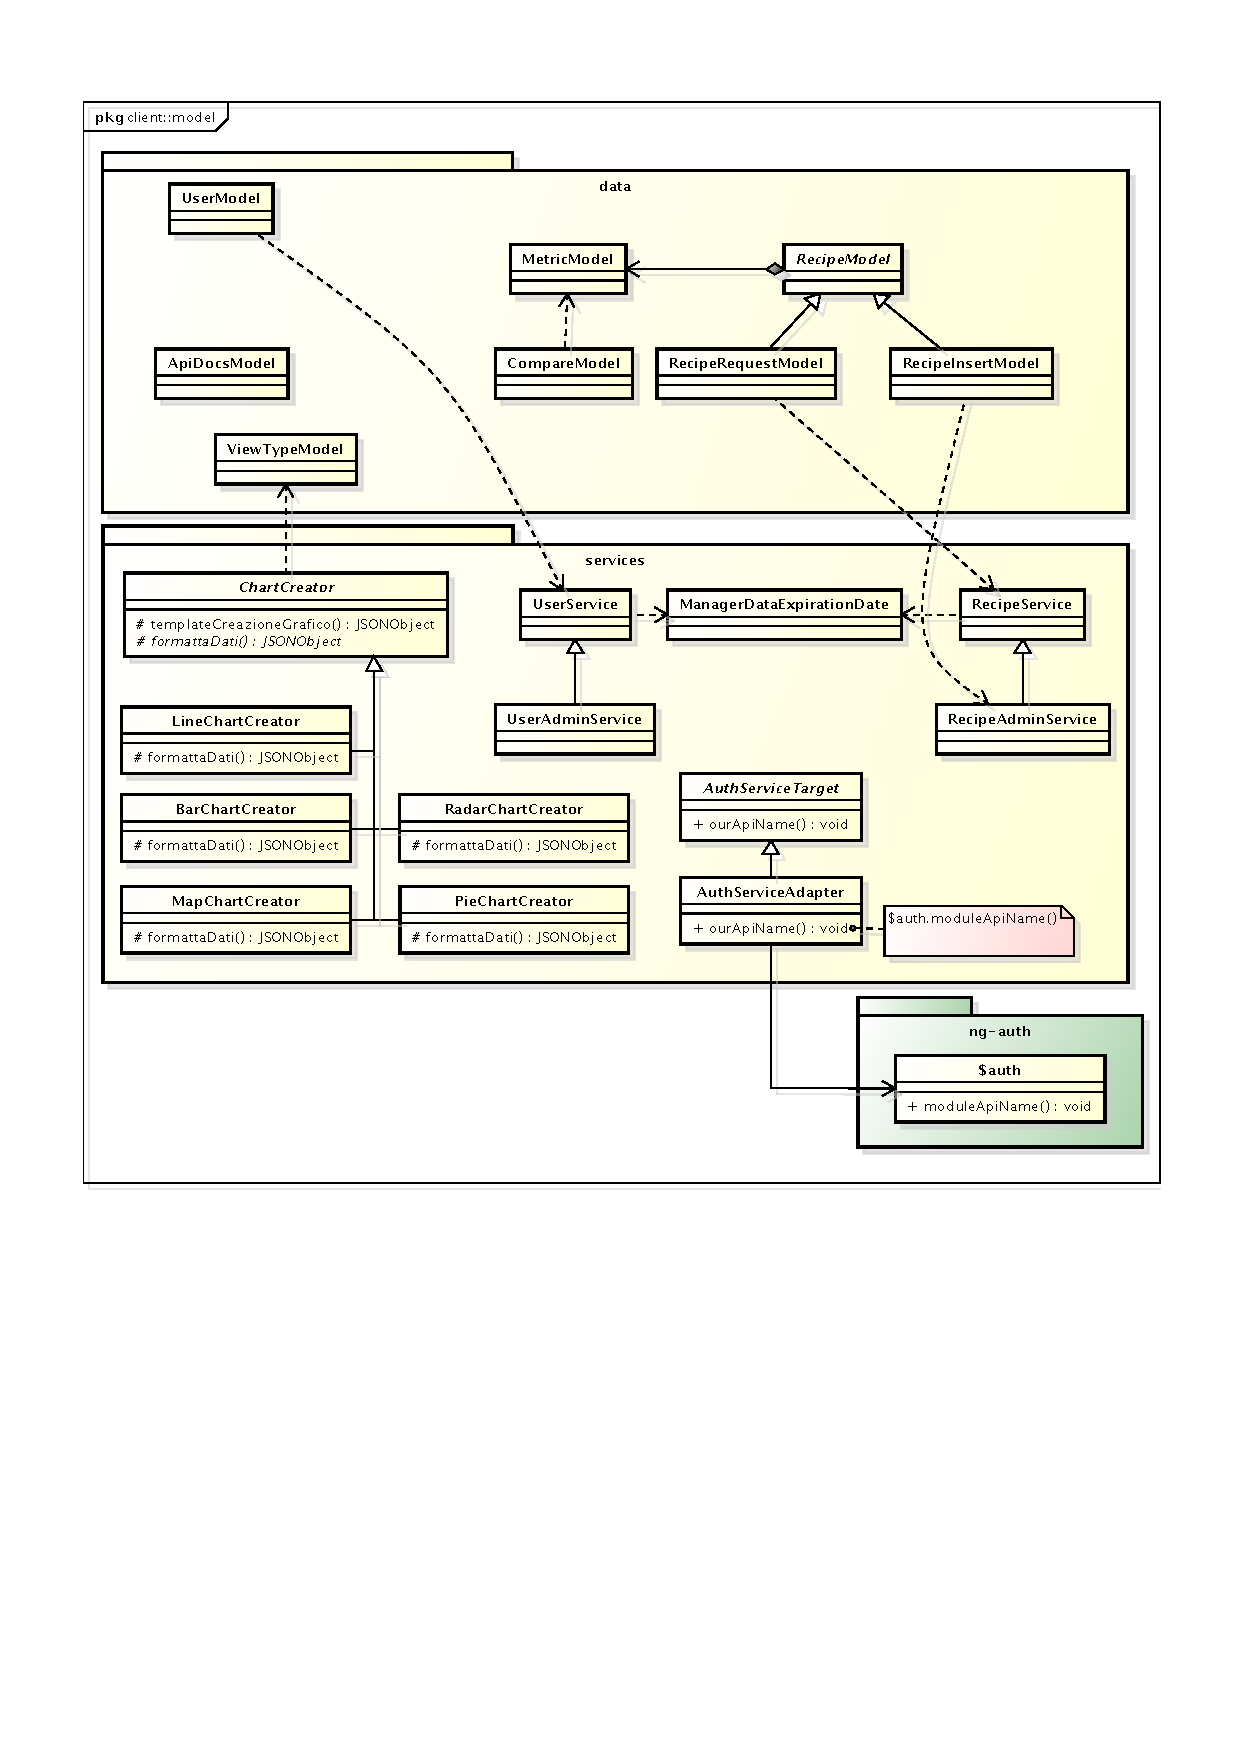
\includegraphics[scale=1.02]{./images/client/client_model.pdf}}
	\caption{Package - client::model}
\end{figure}

\begin{itemize}
	\item \textbf{Descrizione}: è il package che contiene sia le classi dei modelli di dati utilizzati dal client sia i servizi che mettono in comunicazione esso con il server attraverso i diversi servizi REST;
	\item \textbf{Padre}: client;
	\item \textbf{Package contenuti}:
		\begin{itemize}
			\item client::model::data
			\item client::model::services
		\end{itemize}
	\item \textbf{Interazione con altri componenti}:
		\begin{itemize}
			\item client::controller
		\end{itemize}
\end{itemize}
% subsubsection bdsm_app_client_model (end)

% PACKAGE MODEL::DATA
% =================================================================================================
% File:			client_tier/model/data.tex
% Description:	Defiinisce la sezione relativa al front-end dell'applicazione
% Created:		2015-04-10
% Author:		Tesser Paolo
% Email:		tesser.paolo@mashup-unipd.it
% =================================================================================================
% Modification History:
% Version		Modifier Date		Change											Author
% 0.0.1 		2015-04-10 			creato scheletro								Tesser Paolo
% =================================================================================================
% 0.0.2			2015-04-11			scheletro classi contenuti nei package			Tesser Paolo
% =================================================================================================
%

% CONTENUTO DEL CAPITOLO
%

\subsubsection{bdsm\_app::client::model::data} % (fold)
\label{ssub:bdsm_app_client_model_data}
\begin{figure}[htbp]
	\centering
	\centerline{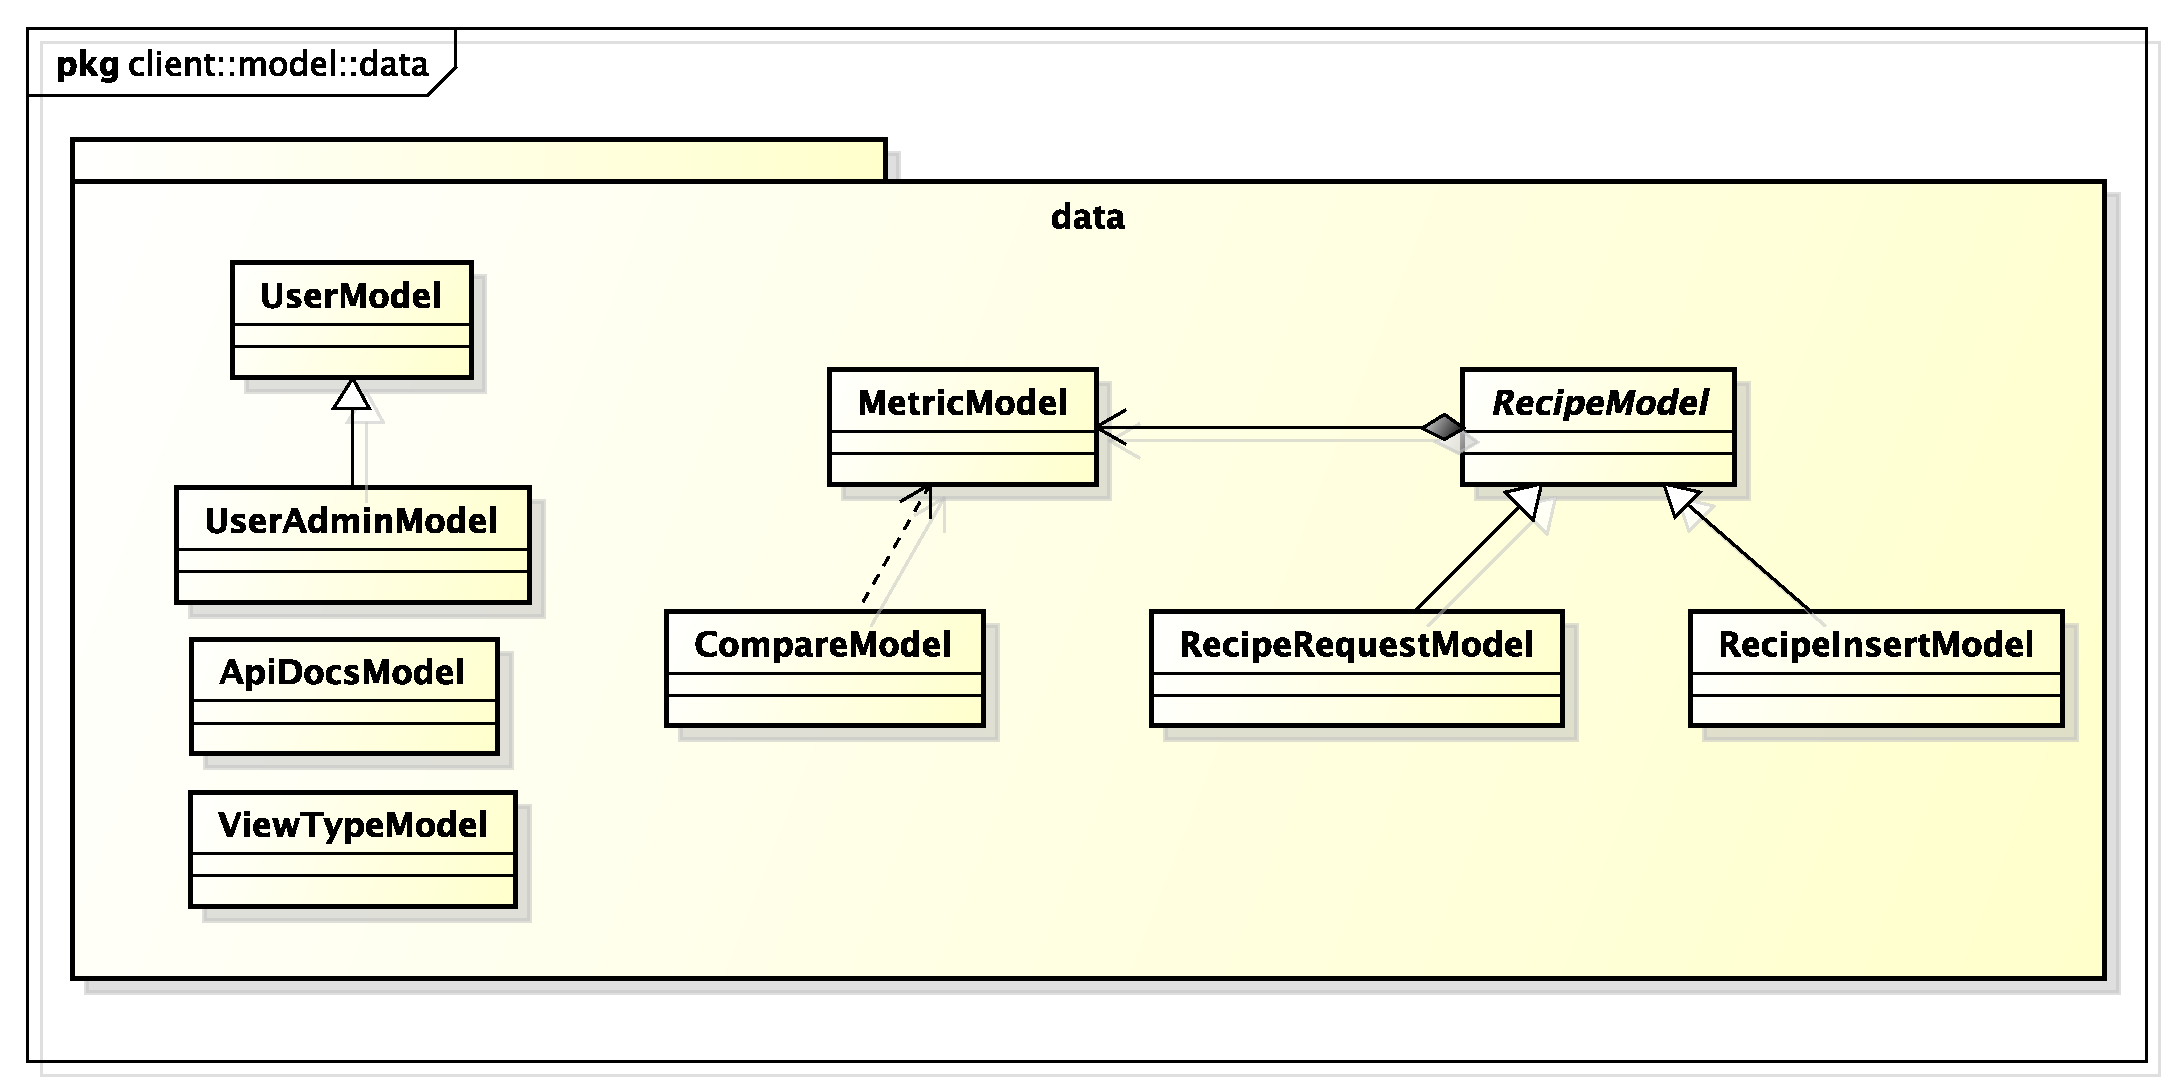
\includegraphics[scale=0.5]{./images/client_model_data.pdf}}
	\caption{Package - client::model::data}
\end{figure}

\begin{itemize}
	\item \textbf{Descrizione}: è il package c;
	\item \textbf{Padre}: client::model
	\item \textbf{Interazione con altri componenti}:
		\begin{itemize}
			\item client::model::services
			\item client::controller
		\end{itemize}

	\paragraph{Classi} % (fold)

		\subparagraph{client::model::data::ViewTypeModel} % (fold)
		\label{subp:client_model_data_viewtypemodel}
			\begin{itemize}
				\item \textbf{Descrizione}: [TO DO];
				\item \textbf{Utilizzo}: [TO DO];
				\item \textbf{Classi ereditate}: [TO DO];
				\item \textbf{Relazioni con altre classi}: [TO DO].
			\end{itemize}
		% subparagraph client_model_data_viewtypedata (end)


		\subparagraph{client::model::data::UserModel} % (fold)
		\label{subp:client_model_data_user}
			\begin{itemize}
				\item \textbf{Descrizione}: [TO DO];
				\item \textbf{Utilizzo}: [TO DO];
				\item \textbf{Classi ereditate}: [TO DO];
				\item \textbf{Relazioni con altre classi}: [TO DO].
			\end{itemize}
		% subparagraph client_model_data_user (end)

		\subparagraph{client::model::data::RecipeModel} % (fold)
		\label{subp:client_model_data_recipe}
			\begin{itemize}
				\item \textbf{Descrizione}: [TO DO];
				\item \textbf{Utilizzo}: [TO DO];
				\item \textbf{Classi ereditate}: [TO DO];
				\item \textbf{Relazioni con altre classi}: [TO DO].
			\end{itemize}
		% subparagraph client_model_data_recipe (end)

		\subparagraph{client::model::data::RecipeRequestModel} % (fold)
		\label{subp:client_model_data_reciperequestmodel}
			\begin{itemize}
				\item \textbf{Descrizione}: [TO DO];
				\item \textbf{Utilizzo}: [TO DO];
				\item \textbf{Classi ereditate}: [TO DO];
				\item \textbf{Relazioni con altre classi}: [TO DO].
			\end{itemize}
		% subparagraph client_model_data_reciperequestmodel (end)

		\subparagraph{client::model::data::RecipeInsertModel} % (fold)
		\label{subp:client_model_data_recipeinsertmodel}
			\begin{itemize}
				\item \textbf{Descrizione}: [TO DO];
				\item \textbf{Utilizzo}: [TO DO];
				\item \textbf{Classi ereditate}: [TO DO];
				\item \textbf{Relazioni con altre classi}: [TO DO].
			\end{itemize}
		% subparagraph client_model_data_recipeinsertmodel (end)

		\subparagraph{client::model::data::MetricModel} % (fold)
		\label{subp:client_model_data_metricmodel}
			\begin{itemize}
				\item \textbf{Descrizione}: [TO DO];
				\item \textbf{Utilizzo}: [TO DO];
				\item \textbf{Classi ereditate}: [TO DO];
				\item \textbf{Relazioni con altre classi}: [TO DO].
			\end{itemize}
		% subparagraph client_model_data_metricmodel (end)


\end{itemize}
% subsubsection bdsm_app_client_model_data (end) % \clearpage \newpage
% END PACKAGE MODEL::DATA

% PACKAGE MODEL::SERVICES
% =================================================================================================
% File:			client_tier/model/services.tex
% Description:	Defiinisce la sezione relativa al front-end dell'applicazione
% Created:		2015-04-10
% Author:		Tesser Paolo
% Email:		tesser.paolo@mashup-unipd.it
% =================================================================================================
% Modification History:
% Version		Modifier Date		Change											Author
% 0.0.1 		2015-04-10 			creato scheletro								Tesser Paolo
% =================================================================================================
%
%

% CONTENUTO DEL CAPITOLO
%

\subsubsection{bdsm\_app::client::model::services} % (fold)
\label{ssub:bdsm_app_client_model_services}
\begin{figure}[htbp]
	\centering
	\centerline{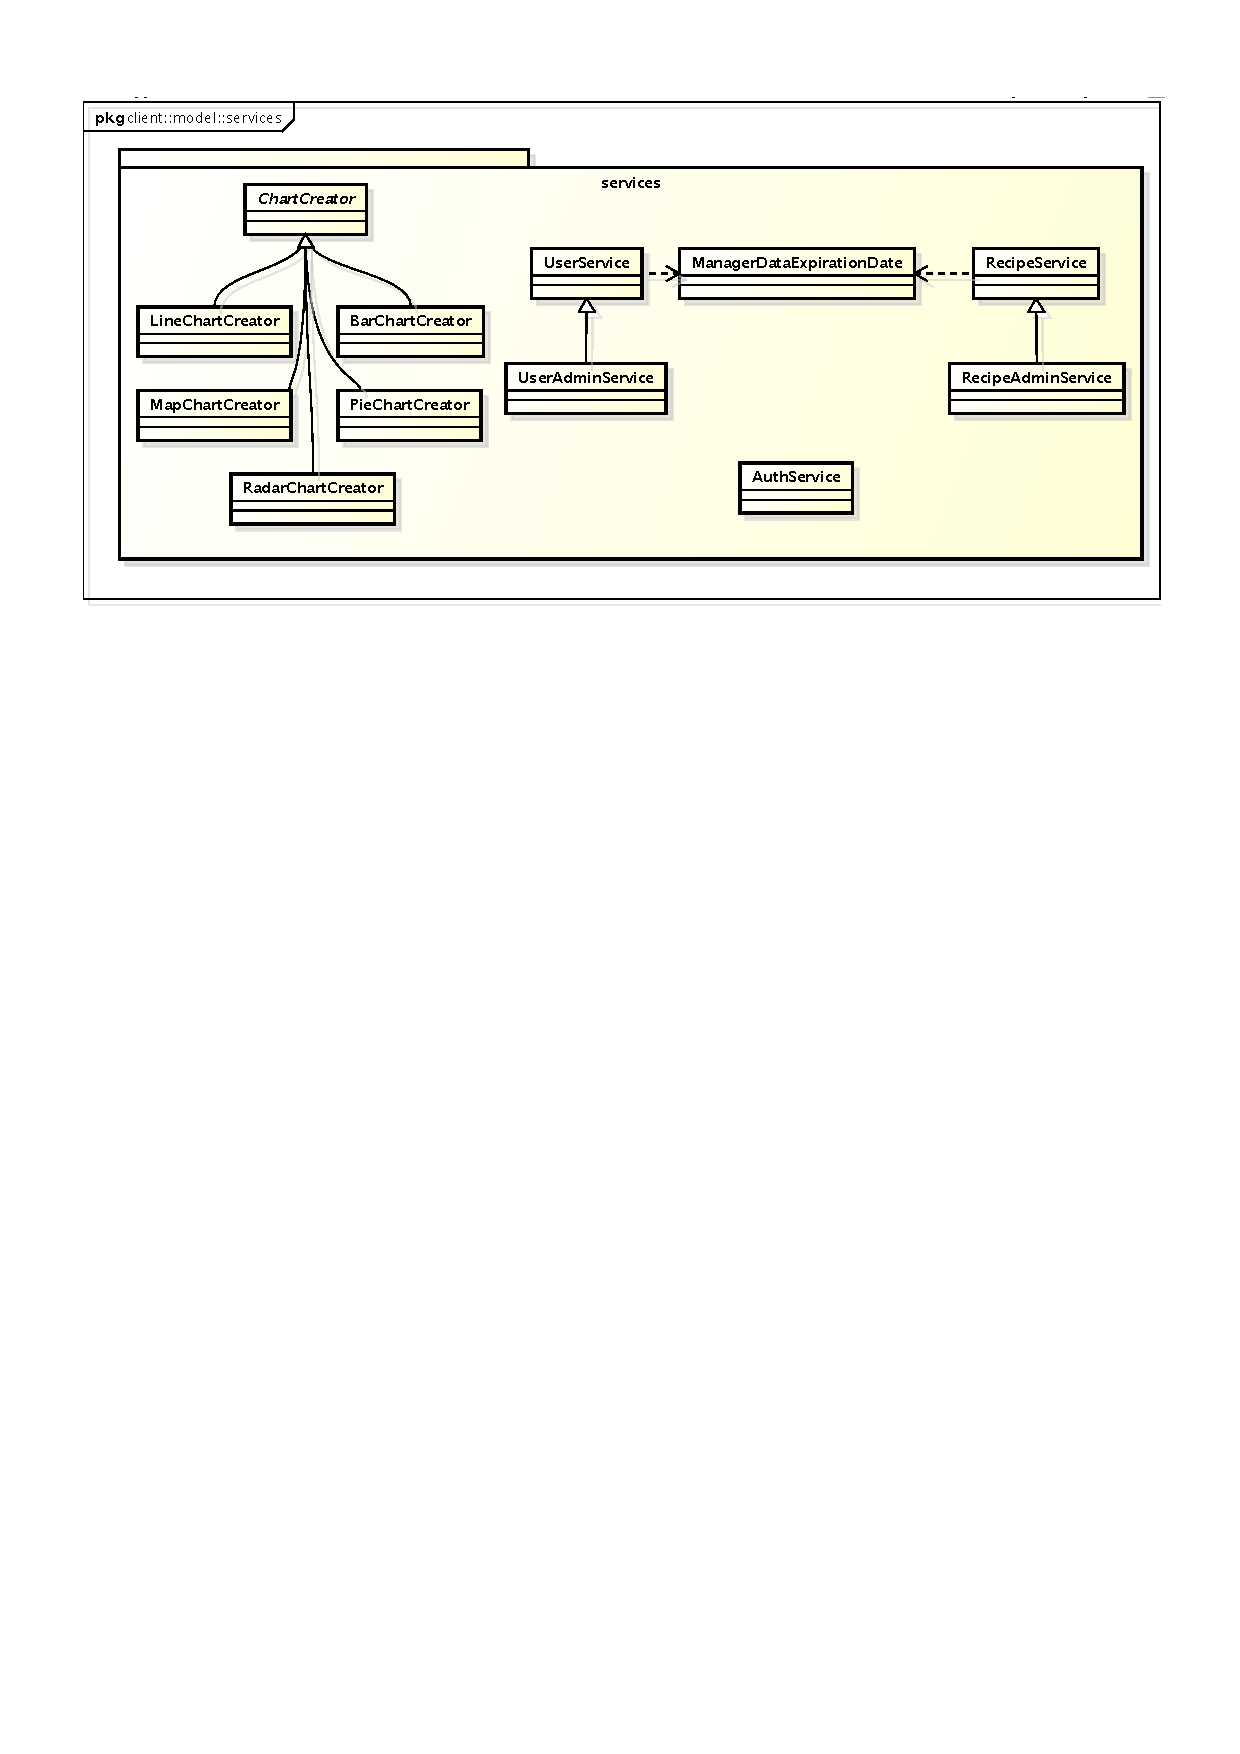
\includegraphics[scale=1.00]{./images/client_model_services.pdf}}
	\caption{Package - client::model}
\end{figure}

\begin{itemize}
	\item \textbf{Descrizione}: È il package che contiene le classi che sviluppano il core business dell'applicazione: in particolare gestiscono il recupero dei dati, siano essi salvati in locale o da recuperare chiamando il server, la crezione dei grafici e l'autenticazione.
	Tutte le classi contenute in questo package implementano il pattern \emph{Singleton};
	\item \textbf{Padre}: client::model
	\item \textbf{Interazione con altri componenti}:
		\begin{itemize}
			\item client::model::data
			\item client::controller
		\end{itemize}
	
	\paragraph{Classi} % (fold)

		\subparagraph{client::model::services::AuthService} % (fold)
		\label{subp:client_model_services_authservice}
			\begin{itemize}
				\item \textbf{Descrizione}: È la classe che implementa un \emph{Adapter} per gestire le chiamate al modulo esterno usato per gestire l'autenticazione;
				\item \textbf{Utilizzo}: I metodi di questa classe saranno invocati quando un utente effettua la registrazione al servizio o effettua un login/logout;
				\item \textbf{Relazioni con altre classi}: 					
					\begin{itemize}
						\item client::controller::public::LoginCtrl
						\item client::controller::public::RegisterCtrl
						\item client::controller::user::LogoutCtrl
					\end{itemize}
			\end{itemize}
		
		\subparagraph{client::model::services::RecipeService} % (fold)
		\label{subp:client_model_services_recipeservice}
			\begin{itemize}
				\item \textbf{Descrizione}: È la classe che racchiude i metodi per reperire i dati relativi alle Recipe, siano essi salvati in locale o da recuperare dal server, inoltre gestisce l'invio di richieste di Recipe al server;
				\item \textbf{Utilizzo}: I suoi metodi vengono invocati ogni volta che sia necessario avere dei dati relativi a una o più Recipe per un utente non amministratore, o se un utente non amministratore desidera inviare una richiesta di Recipe;
				\item \textbf{Relazioni con altre classi}: 					
					\begin{itemize}
						\item client::model::data::RecipeRequestModel
						\item client::model::services::ManagerDataExpirationDate
						\item client::controller::user::RecipeCtrl
						\item client::controller::user::MetricsCtrl
						\item client::controller::user::ChartsCtrl						
						\item client::controller::user::CompareCtrl
					\end{itemize}
			\end{itemize}
		% subparagraph client_model_services_recipeservice (end)

		\subparagraph{client::model::services::RecipeAdminService} % (fold)
		\label{subp:client_model_services_recipeadminservice}
			\begin{itemize}
				\item \textbf{Descrizione}: È la classe che oltre a gestire ciò che è gestito dalla classe padre si occupa dell'inserimento di nuove recipe nel server e dell'eliminazione di Recipe già presenti;
				\item \textbf{Utilizzo}: I suoi metodi vengono invocati quando un utente amministratore desidera agire su dati di Recipe da pagine non accessibili a un utente non amministratore;
				\item \textbf{Classi ereditate}:					
					\begin{itemize}
						\item client::model::services::RecipeService
					\end{itemize}
				\item \textbf{Relazioni con altre classi}:
					\begin{itemize}
						\item client::model::data::RecipeInsertModel
						\item client::model::services::ManagerDataExpirationDate
						\item client::controller::admin::RecipeConfigCtrl
						\item client::controller::admin::InsertRecipeCtrl
					\end{itemize}
			\end{itemize}
		% subparagraph client_model_services_recipeadminservice (end)


		\subparagraph{client::model::services::UserService} % (fold)
		\label{subp:client_model_services_userservice}
			\begin{itemize}
				\item \textbf{Descrizione}: È la classe che gestisce il recupero e la modifica di dati utente relativi a sé stessi;
				\item \textbf{Utilizzo}: I suoi metodi vengono invocati quando un utente accede alla pagina dei propri dati personali;
				\item \textbf{Relazioni con altre classi}:
					\begin{itemize}
						\item client::model::data::UserModel
						\item client::model::services::ManagerDataExpirationDate
						\item client::controller::user::SettingsCtrl
					\end{itemize}
			\end{itemize}
		% subparagraph client_model_services_userservice (end)

		\subparagraph{client::model::services::UserAdminService} % (fold)
		\label{subp:client_model_services_useradminservice}
			\begin{itemize}
				\item \textbf{Descrizione}: È la classe che oltre a gestire ciò che è gestito dalla sua classe padre si occupa del recupero e della modifica di dati di utenti, inclusa l'eliminazione di un utente e il cambiare i suoi permessi;
				\item \textbf{Utilizzo}: I suoi metodi vengono invocati quando un utente amministratore agisce su dati relativi ad utenti da una pagina non accessibile agli utenti non amministratori;
				\item \textbf{Classi ereditate}:					
					\begin{itemize}
						\item client::model::services::UserService
					\end{itemize}
				\item \textbf{Relazioni con altre classi}:
					\begin{itemize}
						\item client::model::data::UserModel
						\item client::model::services::ManagerDataExpirationDate
						\item client::controller::user::UserConfigCtrl
					\end{itemize}
				\end{itemize}
		% subparagraph client_model_services_useradminservice (end)

		\subparagraph{client::model::services::ChartCreator} % (fold)
		\label{subp:chartcreator}
			\begin{itemize}
				\item \textbf{Descrizione}: È una classe astratta che descrive il codice comune delle classi che generano un grafico, secondo il pattern \emph{template method};
				\item \textbf{Utilizzo}: I suoi metodi vengono invocati dalle classi figlie nella creazione di grafici;
				\item \textbf{Relazioni con altre classi}:
					\begin{itemize}
						\item client::model::data::ViewTypeModel
						\item client::model::services::LineChartCreator
						\item client::model::services::BarChartCreator
						\item client::model::services::MapChartCreator
						\item client::model::services::PieChartCreator
						\item client::model::services::RadarChartCreator
						\item client::controller::user::ChartsCtrl
						\item client::controller::user::CompareCtrl
					\end{itemize}
			\end{itemize}
		% subparagraph chartcreator (end)

		\subparagraph{client::model::services::LineChartCreator} % (fold)
		\label{subp:linechartcreator}
			\begin{itemize}
				\item \textbf{Descrizione}: La classe contiene i metodi per la creazione di un Line Chart;
				\item \textbf{Utilizzo}: I suoi metodi vengono invocati quando si vuole creare un Line Chart;
				\item \textbf{Classi ereditate}:					
					\begin{itemize}
						\item client::model::services::ChartCreator
					\end{itemize}
				\item \textbf{Relazioni con altre classi}:					
					\begin{itemize}
						\item client::controller::user::ChartsCtrl
						\item client::controller::user::CompareCtrl
					\end{itemize}
			\end{itemize}
		% subparagraph linechartcreator (end)


		\subparagraph{client::model::services::BarChartCreator} % (fold)
		\label{subp:barchartcreator}
			\begin{itemize}
				\item \textbf{Descrizione}: La classe contiene i metodi per la creazione di un Bar Chart;
				\item \textbf{Utilizzo}: I suoi metodi vengono invocati quando si vuole creare un Bar Chart;
				\item \textbf{Classi ereditate}:					
					\begin{itemize}
						\item client::model::services::ChartCreator
					\end{itemize}
				\item \textbf{Relazioni con altre classi}:					
					\begin{itemize}
						\item client::controller::user::ChartsCtrl
						\item client::controller::user::CompareCtrl
					\end{itemize}
			\end{itemize}
		% subparagraph barchartcreator (end)

		\subparagraph{client::model::services::PieChartCreator} % (fold)
		\label{subp:piechartcreator}
			\begin{itemize}
				\item \textbf{Descrizione}: La classe contiene i metodi per la creazione di un Pie Chart;
				\item \textbf{Utilizzo}: I suoi metodi vengono invocati quando si vuole creare un Pie Chart;
				\item \textbf{Classi ereditate}:					
					\begin{itemize}
						\item client::model::services::ChartCreator
					\end{itemize}
				\item \textbf{Relazioni con altre classi}:					
					\begin{itemize}
						\item client::controller::user::ChartsCtrl
						\item client::controller::user::CompareCtrl
					\end{itemize}
			\end{itemize}
		% subparagraph piechartcreator (end)

		\subparagraph{client::model::services::MapChartCreator} % (fold)
		\label{subp:mapchartcreator}
			\begin{itemize}
				\item \textbf{Descrizione}: La classe contiene i metodi per la creazione di un Map Chart;
				\item \textbf{Utilizzo}: I suoi metodi vengono invocati quando si vuole creare un Map Chart;
				\item \textbf{Classi ereditate}:					
					\begin{itemize}
						\item client::model::services::ChartCreator
					\end{itemize}
				\item \textbf{Relazioni con altre classi}:					
					\begin{itemize}
						\item client::controller::user::ChartsCtrl
						\item client::controller::user::CompareCtrl
					\end{itemize}
			\end{itemize}
		% subparagraph mapchartcreator (end)

		\subparagraph{client::model::services::RadarChartCreator} % (fold)
		\label{subp:radarchartcreator}
			\begin{itemize}
				\item \textbf{Descrizione}: La classe contiene i metodi per la creazione di un Radar Chart;
				\item \textbf{Utilizzo}: I suoi metodi vengono invocati quando si vuole creare un Radar Chart;
				\item \textbf{Classi ereditate}:					
					\begin{itemize}
						\item client::model::services::ChartCreator
					\end{itemize}
				\item \textbf{Relazioni con altre classi}:					
					\begin{itemize}
						\item client::controller::user::ChartsCtrl
						\item client::controller::user::CompareCtrl
					\end{itemize}
			\end{itemize}
		% subparagraph radarchartcreator (end)

		\subparagraph{client::model::services::ManagerDataExpirationDate} % (fold)
		\label{subp:radarchartcreator}
			\begin{itemize}
				\item \textbf{Descrizione}: Questa classe controlla se i dati che vengono richiesti sono già presenti in locale o se devono essere richiesti al server: in particolare li richiede al server solo se questi sono assenti o se sono l'ultima volta che sono stati chiesti al server è passata da troppo tempo;
				\item \textbf{Utilizzo}: I suoi metodi vengono invocati dalle classi che desiderano fare richieste al server;
				\item \textbf{Relazioni con altre classi}:					
					\begin{itemize}
						\item client::model::services::RecipeService
						\item client::model::services::RecipeAdminService
						\item client::model::services::UserService
						\item client::model::services::UserAdminService
					\end{itemize}
			\end{itemize}
		% subparagraph managerdataexpirationdate (end)


\end{itemize}
% subsubsection bdsm_app_client_model_services (end)
% END PACKAGE MODEL::SERVICES
